\documentclass[a4paper, 12pt]{article}
\usepackage[utf8]{inputenc}
\usepackage{amsmath}
\usepackage{amssymb}
\usepackage{lscape}
\usepackage{graphics}
\usepackage{graphicx}
\usepackage{color}
\usepackage{array}
\usepackage{hyperref}
\usepackage{float}
\usepackage[english]{babel}
\usepackage[T1]{fontenc}
\usepackage[a4paper, total={6in, 10in}]{geometry}
\usepackage{stackengine} 
\usepackage{siunitx}
\usepackage{tabularx}
\usepackage{imakeidx}
\usepackage{caption}
\usepackage{subcaption}
\usepackage{pdfpages}
\usepackage{adjustbox}
\usepackage{eurosym}
\usepackage{longtable}
\usepackage{enumitem}
\setlength{\parindent}{0pt}

% Start the document
\begin{document}

% Title page
\begin{titlepage}
    \centering
    \begin{figure}[H]
	    
\includegraphics[width = 6in]{Figures/Logo_Univ.png}
    \end{figure}

    \vspace*{5cm}

    \rule{\textwidth}{2pt}
    \vspace{0.5cm}

    {\fontsize{30}{30}\selectfont \textbf{Design and Implementation of a Modular 
    Dual-Evaporator Transcritical High Temperature Heat Pump}}

    \vspace{1cm}

    {\LARGE Catalogue of Possible Cycle Configurations}

    \vspace{0.5cm}
    \rule{\textwidth}{2pt}


    \vspace{1cm}

    %\begin{figure}[H]
    %    \centering
    %    
\includegraphics[width = 3.5in]{Figures/ST.png}
    %\end{figure}

    \vfill

    {\large \textbf{Authors:} \\
    Franklin Grégoire \\
    Hugo Warscotte}

    \vspace{1cm}

    {\large \textbf{Date:} \today}

    \vspace{1cm}
    
    {\large \textbf{Ecole Polytechnique de Louvain}}

\end{titlepage}

\newpage

\vspace*{2cm}

\section*{Abstract}
\begin{center}
    This document presents the various possible cycle 
configurations for the modular high-temperature heat pump (HTHP) system, 
along with their corresponding schematics and specified boundary conditions.

% Remark : We could also add T-s and P-h diagrams for each cycle configuration.

\end{center}

\vspace{1cm}

\renewcommand{\contentsname}{Table of Contents}
\tableofcontents

\vfill

\rule{\textwidth}{2pt}

\section*{Note on AI assistance}
This document was proofread with the assistance of \texttt{ChatGPT}, 
an AI language model developed by \texttt{OpenAI}.

\vspace{1cm}
\newpage

\section{Subcritical Cycles}

\subsection{One Evaporator - SC1}
The schematic for the One Evaporator Subcritical Heat Pump cycle (SC1) is shown 
in Figure \ref{fig:SC1}.

\begin{figure}[H]
    \centering
    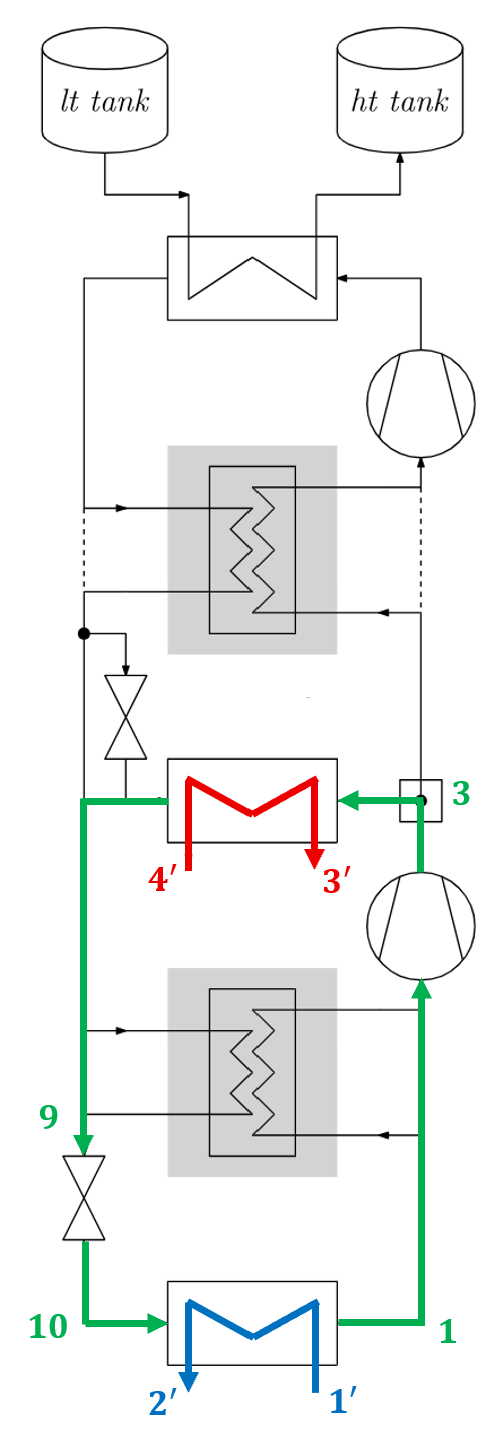
\includegraphics[width=0.35\textwidth]{Figures/SC1.png}
    \begin{minipage}{0.7\textwidth}
        \caption{Schematic of the One Evaporator Subcritical Heat Pump cycle (SC1)}
        \label{fig:SC1}
    \end{minipage}
\end{figure}

\textcolor{red}{To be completed}

\newpage

\subsection{One Evaporator with Recuperator - SC1R}
The schematic for the One Evaporator Subcritical Heat Pump cycle with Recuperator (SC1R) is shown 
in Figure \ref{fig:SC1R}.

\begin{figure}[H]
    \centering
    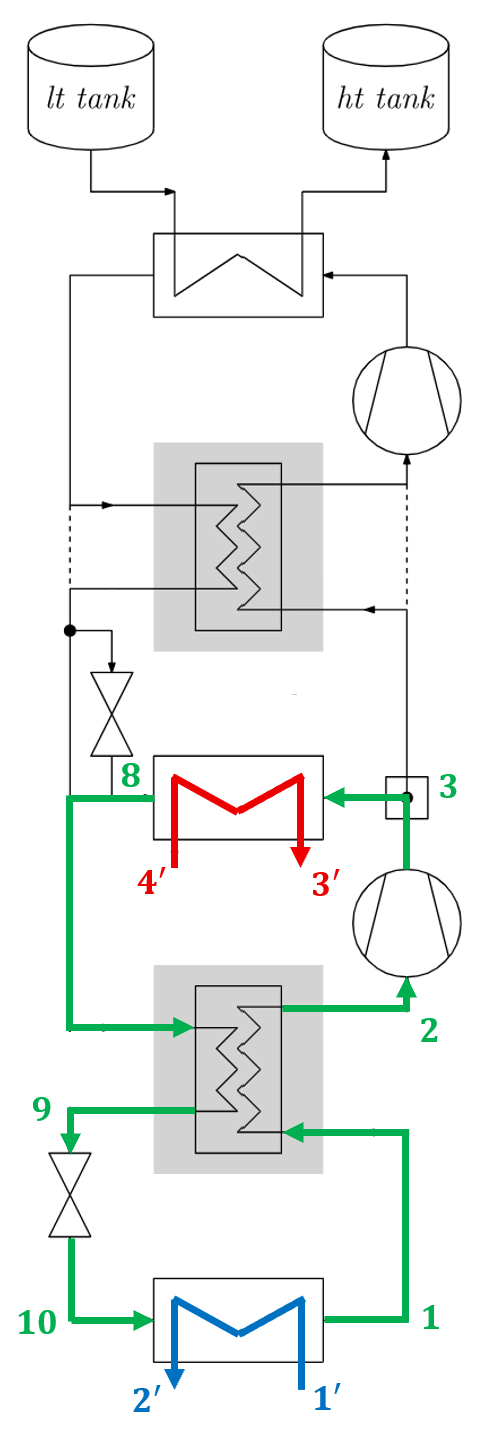
\includegraphics[width=0.35\textwidth]{Figures/SC1R.png}
    \begin{minipage}{0.7\textwidth}
        \caption{Schematic of the One Evaporator Subcritical Heat Pump cycle with Recuperator (SC1R)}
        \label{fig:SC1R}
    \end{minipage}
\end{figure}

\textcolor{red}{To be completed}

\newpage

\subsection{Two Evaporators - SC2}
The schematic for the Dual-Evaporator Subcritical Heat Pump cycle (SC2) is shown 
in Figure \ref{fig:SC2} and the corresponding operating conditions are summarized in Table 
\ref{tab:SC2_conditions}.

\begin{figure}[H]
    \centering
    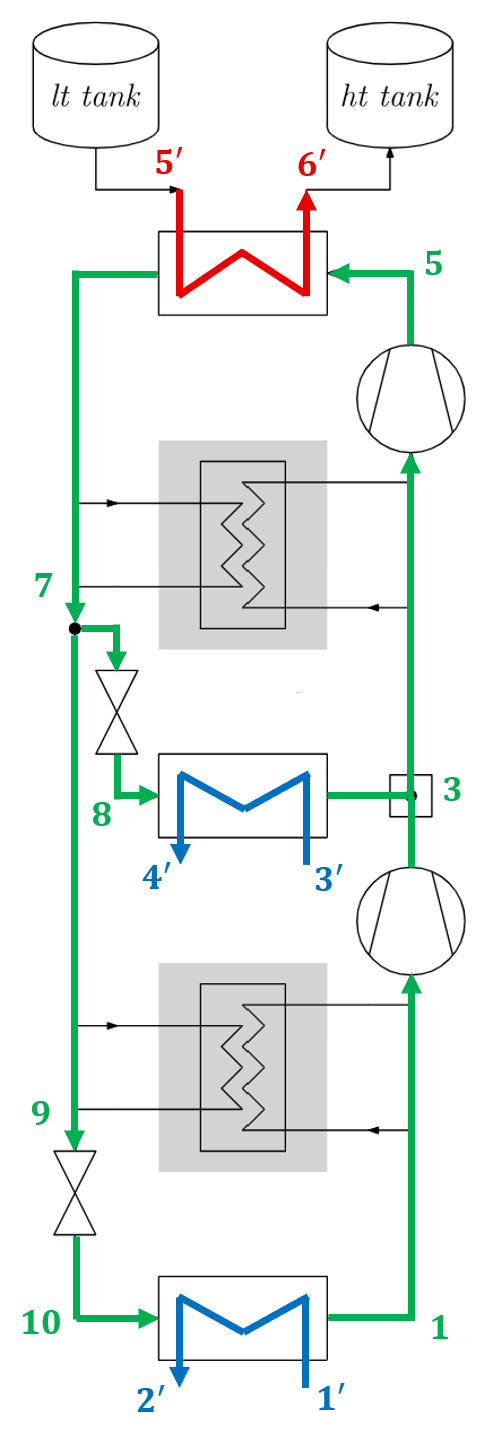
\includegraphics[width=0.35\textwidth]{Figures/SC2.png}
    \begin{minipage}{0.7\textwidth}
        \caption{Schematic of the Dual-Evaporator Subcritical Heat Pump cycle (SC2) 
        (\textit{green: working fluid; blue: heat source(s); red: heat sink})}
        \label{fig:SC2}
    \end{minipage}
\end{figure}

\begin{table}[H]
\centering
\begin{tabular}{|c|c|c|c|}
\hline
\textbf{LT heat source} & \textbf{MT heat source} & \textbf{Working fluid} & \textbf{Heat sink} \\
\hline
Water & Water & R290 (propane) & Water \\
%\hline
$T_{1}' = 10\,^{\circ}\mathrm{C}$ & $T_{3}' = 40\,^{\circ}\mathrm{C}$ & -- & $T_{5}' = 60\,^{\circ}\mathrm{C}$ \\
%\hline
$\dot{m}_\mathrm{c} = 0.4\,\mathrm{kg/s}$ & $\dot{m}_\mathrm{c} = 1.2\,\mathrm{kg/s}$ & -- & $\dot{m}_\mathrm{h} = 1\,\mathrm{kg/s}$ \\
\hline
\end{tabular}
\caption{Operating conditions for the SC2 cycle}
\label{tab:SC2_conditions}
\end{table}

\newpage

\subsection{Two Evaporators with Recuperators - SC2R}
The schematic for the Dual-Evaporator Subcritical Heat Pump cycle with Recuperators (SC2R) is shown 
in Figure \ref{fig:SC2R}.

\begin{figure}[H]
    \centering
    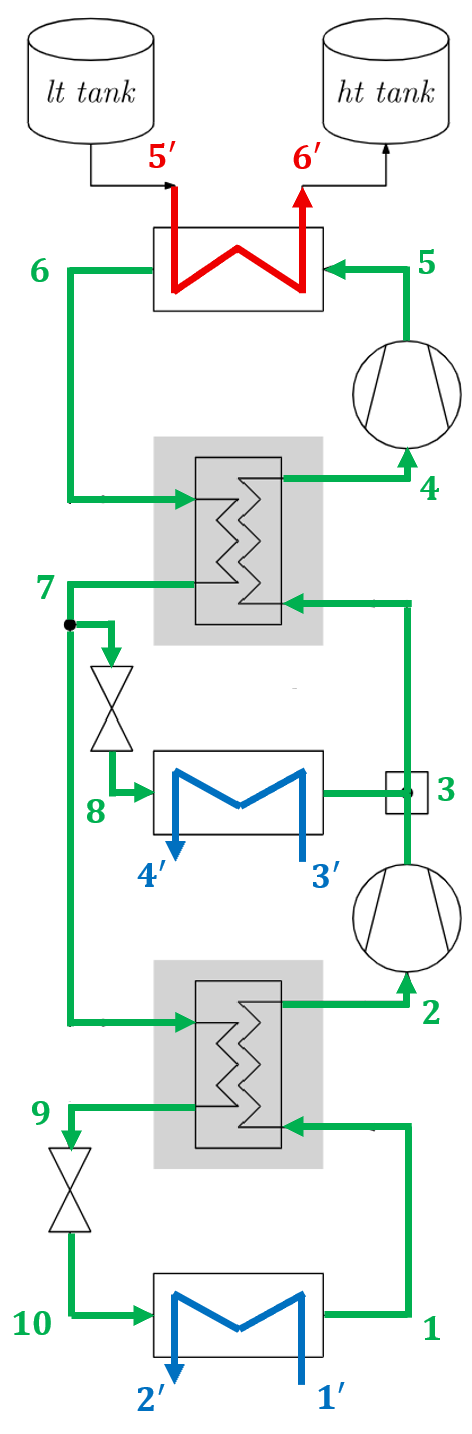
\includegraphics[width=0.35\textwidth]{Figures/SC2R.png}
    \begin{minipage}{0.7\textwidth}
        \caption{Schematic of the Dual-Evaporator Subcritical Heat Pump cycle with Recuperator (SC2R)}
        \label{fig:SC2R}
    \end{minipage}
\end{figure}

\textcolor{red}{To be completed}

\newpage

\section{Transcritical Cycles}

\subsection{One Evaporator - TC1}
The schematic for the One Evaporator Transcritical Heat Pump cycle (TC1) is shown 
in Figure \ref{fig:TC1} and the corresponding operating conditions are summarized in Table 
\ref{tab:TC1_conditions}.

\begin{figure}[H]
    \centering
    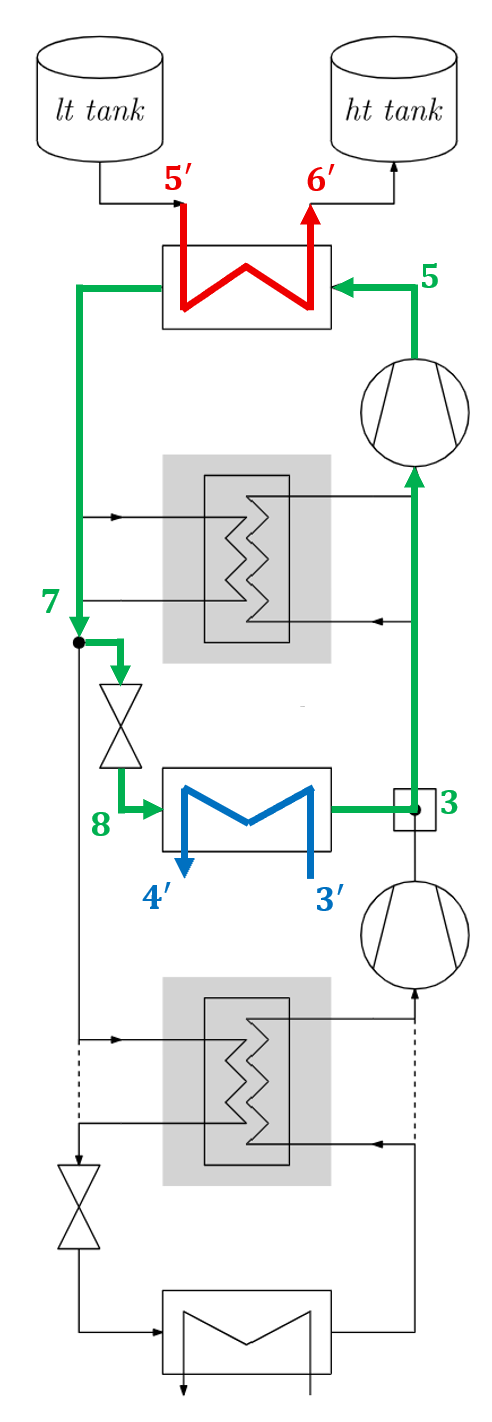
\includegraphics[width=0.35\textwidth]{Figures/TC1.png}
    \begin{minipage}{0.7\textwidth}
        \caption{Schematic of the One Evaporator Transcritical Heat Pump cycle (TC1) 
        (\textit{green: working fluid; blue: heat source(s); red: heat sink})}
        \label{fig:TC1}
    \end{minipage}
\end{figure}

\begin{table}[H]
\centering
\begin{tabular}{|c|c|c|c|}
\hline
 & \textbf{Heat source} & \textbf{Working fluid} & \textbf{Heat sink} \\
\hline
Fluid & Water & R290 (propane) & Water \\
%\hline
Inlet temperature & $T_{3}' = 40\,^{\circ}\mathrm{C}$ & -- & $T_{5}' = 60\,^{\circ}\mathrm{C}$ \\
%\hline
Mass flow rate & $\dot{m}_\mathrm{c} = 0.5\,\mathrm{kg/s}$ & -- & $\dot{m}_\mathrm{h} = 0.1\,\mathrm{kg/s}$ \\
\hline
\end{tabular}
\caption{Operating conditions for the TC1 cycle}
\label{tab:TC1_conditions}
\end{table}

%\textbf{Note:} The heat sink mass flow rate is lower than 
%in the SC2 cycle to increase the temperature glide, 
%as transcritical cycles generally perform better with 
%larger temperature differences compared to subcritical cycles.
\newpage

\subsection{One Evaporator with Recuperator - TC1R}
The schematic for the One Evaporator Transcritical Heat Pump cycle with Recuperator (TC1R) is shown 
in Figure \ref{fig:TC1R}.

\begin{figure}[H]
    \centering
    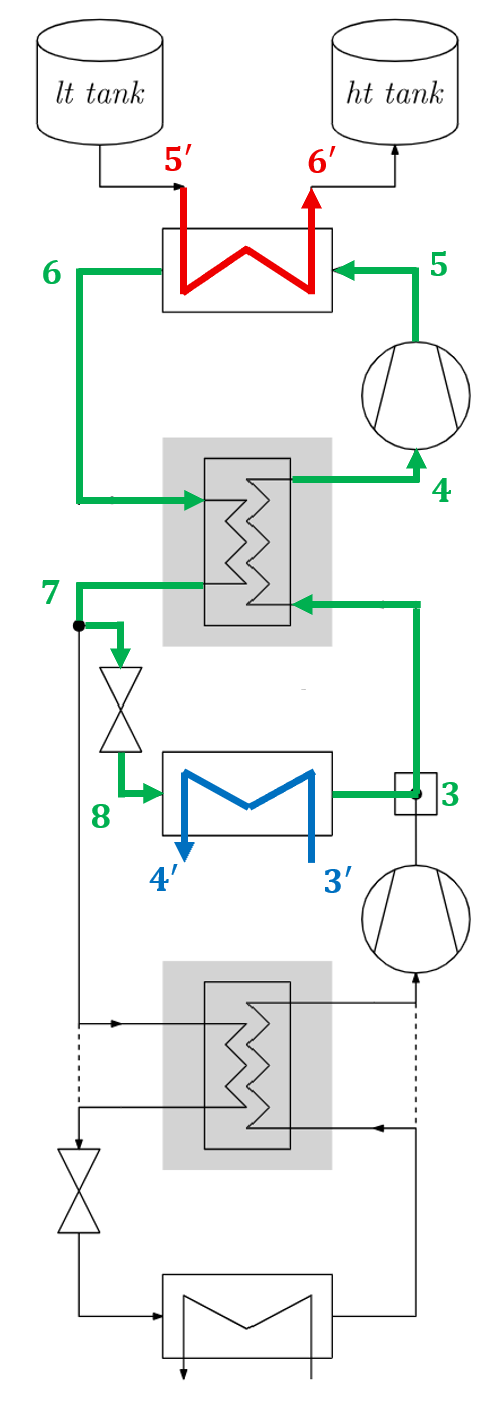
\includegraphics[width=0.35\textwidth]{Figures/TC1R.png}
    \begin{minipage}{0.7\textwidth}
        \caption{Schematic of the One Evaporator Transcritical Heat Pump cycle with Recuperator (TC1R)}
        \label{fig:TC1R}
    \end{minipage}
\end{figure}

\textcolor{red}{To be completed}

\newpage

\subsection{Two Evaporators - TC2}
The schematic for the Dual-Evaporator Transcritical Heat Pump cycle (TC2) is shown 
in Figure \ref{fig:TC2}.

\begin{figure}[H]
    \centering
    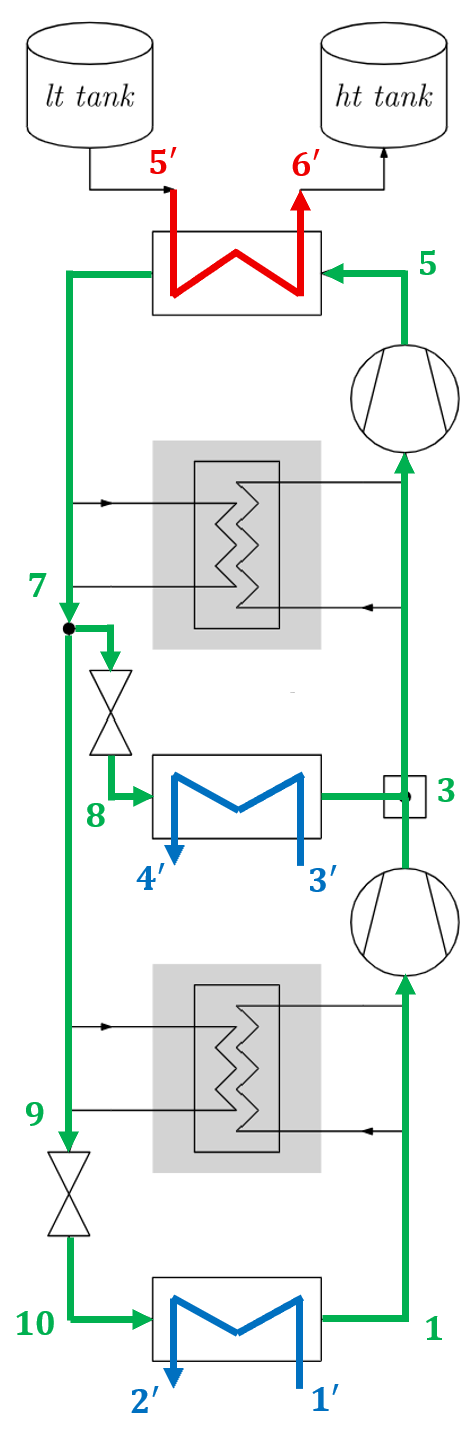
\includegraphics[width=0.35\textwidth]{Figures/TC2.png}
    \begin{minipage}{0.7\textwidth}
        \caption{Schematic of the Dual-Evaporator Transcritical Heat Pump cycle (TC2)}
        \label{fig:TC2}
    \end{minipage}
\end{figure}

\textcolor{red}{To be completed}

\newpage

\subsection{Two Evaporators with Recuperators - TC2R}
The schematic for the Dual-Evaporator Transcritical Heat Pump cycle with Recuperators (TC2R) is shown 
in Figure \ref{fig:TC2R}.

\begin{figure}[H]
    \centering
    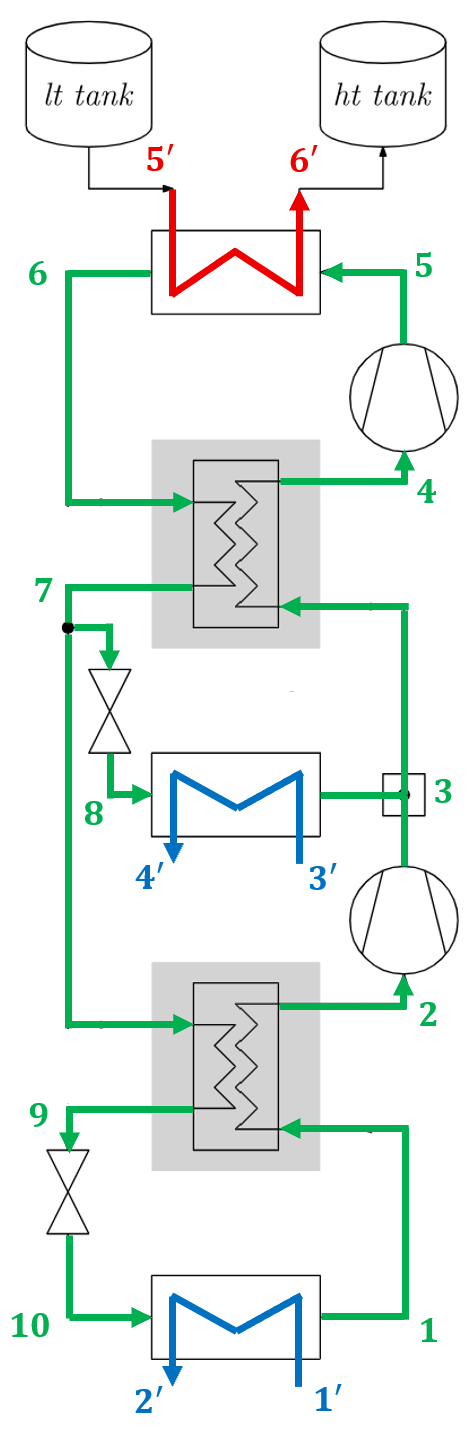
\includegraphics[width=0.35\textwidth]{Figures/TC2R.png}
    \begin{minipage}{0.7\textwidth}
        \caption{Schematic of the Dual-Evaporator Transcritical Heat Pump cycle with Recuperator (TC2R)}
        \label{fig:TC2R}
    \end{minipage}
\end{figure}

\textcolor{red}{To be completed}

\newpage

\newpage
\section{Notes}
One can note the following regarding the operating conditions of the cycles:

\begin{itemize}
    \item For cycles with two evaporators, the mass flow rate at the 
    low-temperature heat source is always one-third of the mass flow    
    rate at the medium-temperature heat source. Assuming the same 
    temperature difference at both evaporators, this ensures that $\beta \approx 75\%$.
    \item For transcritical cycles, the mass flow rate at the heat 
    sink is always lower than for subcritical cycles. This adjustment 
    increases the temperature glide at the heat sink, highlighting 
    one of the key advantages of transcritical operation.
\end{itemize}


\newpage

%\bibliographystyle{plain} % We choose the "plain" reference style
%\nocite{*}
%\bibliography{src/refs} % Entries are in the refs.bib file

%\section*{}

%\newpage

%\appendix
%\section*{Appendix}

\end{document}
